\documentclass[letterpaper, 10pt]{article}

\usepackage{amsfonts}
\usepackage{amsmath}
\usepackage{hyperref}
\usepackage{xcolor}
\usepackage[UTF8]{ctex}
\usepackage{geometry}
\usepackage{fontspec}
\usepackage{graphicx}
\usepackage{subfigure}

\geometry{left=2cm,right=2cm,top=2cm,bottom=2cm}
\hypersetup{
	colorlinks, linkcolor=blue, anchorcolor=blue, citecolor=blue
}

\newcommand{\qbar}{\rangle}
\newcommand{\qket}{\langle}
\newcommand{\dd}{\mathrm{d}}
\newcommand{\dbar}{\mathrm{d}\hspace*{-0.18em}\bar{}\hspace*{0.2em}}

\begin{document}

\title{热统习题的部分答案(野生版)}
\author{}
\date{\today}
\maketitle
\thispagestyle{empty}

\tableofcontents

\newpage
\setcounter{page}{1}


\section[第一章]{第一章}

\subsection{习题1.6}
\begin{eqnarray*}
\alpha = \frac{1}{V} \left( \frac{\partial V}{\partial T} \right)_{p} = \frac{\nu R}{pV} & \Rightarrow & \left( \frac{\partial V}{\partial T} \right)_{p} = \frac{\nu R}{p} \\
& \Rightarrow & V = \frac{\nu R T}{p} + g(p) \quad{} \text{代入$ \kappa = \frac{1}{p} + \frac{a}{V} = - \frac{1}{V} \left( \frac{\partial V}{\partial p} \right)_{T} $} \\
& \Rightarrow & \dd( p g(p) ) = - \frac{a}{2} \dd ( p^2 ) \\
& \Rightarrow & p g(p) = - \frac{a}{2} p^2 + \mathrm{const} \quad{} \text{代入第二行式子并整理} \\
& \Rightarrow & pV = \nu RT - \frac{a}{2} p^2 + \mathrm{const} \,.
\end{eqnarray*}

\subsection{习题1.8}
\begin{itemize}
	\item[1)]
	利用广延量假设,
	\begin{eqnarray*}
	S = Ns, V = Nv, U = Nu & \Rightarrow & s = A(vu)^{1/3} \\
	&\Rightarrow & T \dd s = T A \frac{v \dd u + u \dd v}{3(vu)^{2/3}} = \dd u + p \dd v \\
	\text{$\dd u, \dd v$前的系数对应相等并恢复广延量} & \Rightarrow & 		 	
		\begin{cases}
		T = \frac{3u^{2/3}}{Av^{1/3}} = \frac{3U^{2/3}}{A(NV)^{1/3}} \quad{} \text{易得: $ U \sim T^{3/2} $} \\
		p = \left( \frac{N}{V} \right)^{1/2} \left( \frac{AT}{3} \right)^{3/2}
		\end{cases} \\
	\end{eqnarray*}
	\[ C_{V} = \left( \frac{\partial U}{\partial T} \right)_{V} = \frac{1}{2} \sqrt{\frac{A^3 NVT}{3}} \quad{} \text{利用了前面的温度表达式.} \]
	\item[2)]
	对于每个热源而言, 我们有: 
	\[ \dbar Q = \dd U \sim T^{1/2} \dd T, \]
	由于高温热源放出热量($ \Delta Q_{h} < 0 $)必定大于等于低温热源吸热($ \Delta Q_{c} > 0 $), 不失一般性, 我们假设$ T_{1} > T_{2} $, 
	\begin{eqnarray*}
	\Delta Q_{h} + \Delta Q_{c} \leq 0 & \Rightarrow & \left( \int_{T_{1}}^{T_{f}} + \int_{T_{2}}^{T_{f}} \right) T^{1/2} \dd T \leq 0 \\
	& \Rightarrow & T_{f} \leq \left( \frac{T_{1}^{3/2} + T_{2}^{3/2}}{2} \right)^{2/3} \,;
	\end{eqnarray*}
	另一方面, 由热力学第二定律: $ \Delta S \geq 0 $,
	\begin{eqnarray*}
	\Delta S = \left( \int_{T_{1}}^{T_{f}} + \int_{T_{2}}^{T_{f}} \right) \frac{\dbar Q}{T} 
	\sim \left( \int_{T_{1}}^{T_{f}} + \int_{T_{2}}^{T_{f}} \right) \frac{1}{T^{1/2}} \dd T \geq 0 \\
	\Rightarrow \quad{} T_{f} \geq \left( \frac{T_{1}^{1/2}+T_{2}^{1/2}}{2} \right)^{2} \,.
	\end{eqnarray*}
	由第一题的温度表达式, 我们得到: 
	\[ U = \left( \frac{AT(NV)^{1/3}}{3} \right)^{3/2} = C T^{3/2}. \]
	对于整个系统而言,
	\[ W = - \Delta U_{\text{总}} = C \left( T_{1}^{3/2} + T_{2}^{3/2} - 2 T_{f}^{3/2} \right) \leq \sqrt{\frac{A^{3}NV}{27}} 
	\left[ T_{1}^{3/2} + T_{2}^{3/2} - 2 \left( \frac{T_{1}^{1/2}+T_{2}^{1/2}}{2} \right)^3 \right] \,. \]
\end{itemize}

\subsection{习题1.11}
首先,我们需要求出范氏气体的内能表达式, 
\begin{eqnarray*}
\text{由范氏气体的状态方程} & \Rightarrow & \left( \frac{\partial p}{\partial T} \right)_{V} = \frac{R}{V-b} \\
\text{代入书上式子($ 1.9.16 $)} & \Rightarrow & 
\left( \frac{\partial U}{\partial V} \right)_{T} = - p + T \left( \frac{\partial p}{\partial T} \right)_{V} = \frac{a}{V^{2}} \\
& \Rightarrow & \dd U = C_{V} \dd T + \left( \frac{\partial U}{\partial V} \right)_{T} \dd V = C_{V} \dd T + \frac{a}{V^{2}} \dd V \\
& \Rightarrow & U = C_{V} T - \frac{a}{V} + U_{0} \,.
\end{eqnarray*}
\begin{itemize}
	\item[1)]
	对于等温过程,
	\begin{align*}
	& \Delta U = - \frac{a}{V_{f}} + \frac{a}{V_{i}} \\
	& W = \int_{V_{i}}^{V_{f}} p \dd V = \int_{V_{i}}^{V_{f}} \left( \frac{RT_{i}}{V-b} - \frac{a}{V^2} \right) \dd V = 
	RT_{i} \ln \left( \frac{V_{f}-b}{V_{i}-b} \right) + \frac{a}{V_{f}} - \frac{a}{V_{i}} \\
	& \Delta S = \frac{\Delta U + W}{T_{i}} = R \ln \frac{V_{f}-b}{V_{i}-b} \,;
	\end{align*}
	\item[2)]
	对于等压过程, 
	\[ W = p_{i} (V_{f} - V_{i}) = \left( \frac{RT_{i}}{V_{i}-b} - \frac{a}{V_{i}^2} \right) (V_{f} - V_{i}) \]
	\begin{eqnarray*}
	\text{利用状态方程} & \Rightarrow & T_{f} = \left( p_{i} + \frac{a}{V_{f}^2} \right)(V_{f} - b)/R = 
	\left( \frac{RT_{i}}{V_{i}-b} - \frac{a}{V_{i}^2} + \frac{a}{V_{f}^2} \right)(V_{f} - b)/R \\
	& \Rightarrow & \Delta U = C_{V}(T_{f} - T_{i}) - \frac{a}{V_{f}} + \frac{a}{V_{i}} = 
	C_{V}\left[ \left( \frac{RT_{i}}{V_{i}-b} - \frac{a}{V_{i}^2} + \frac{a}{V_{f}^2} \right)(V_{f} - b)/R - T_{i} \right] - \frac{a}{V_{f}} + \frac{a}{V_{i}}
	\end{eqnarray*}
	\begin{eqnarray*}
	\text{由等压条件} & \Rightarrow & T \dd S = \dbar Q = C_{p} \dd T \\
	& \Rightarrow & \dd S = C_{p} \dd(\ln T) \\
	& \Rightarrow & \Delta S = C_{p} \ln \frac{T_{f}}{T_{i}} = C_{p} \ln 
	\left[ \frac{V_{f}-b}{V_{i}-b} - a\left( \frac{1}{V_{i}^2} - \frac{1}{V_{f}^2} \right) \frac{V_{f}-b}{RT_{i}} \right] \,;
	\end{eqnarray*}
	\item[3)]
	对于绝热过程, 
	\[ \dbar Q = \dd U + p \dd V = \left( \frac{\partial U}{\partial T} \right)_{V} \dd T + 
	\left[ \left( \frac{\partial U}{\partial V} \right)_{T} + p \right] \dd V = C_{V} \dd T + \left( \frac{a}{V^{2}} + p \right) \dd V = 0 \,, \]
	\begin{eqnarray*}
	\text{结合状态方程} & \Rightarrow & C_{V} \dd T + \frac{RT}{V-b} \dd V = 0 \\
	& \Rightarrow & C_{V} \ln T + R \ln (V-b) = 0 \\
	& \Rightarrow & T^{C_{V}} (V-b)^{R} = \mathrm{const} \\
	& \Rightarrow & T_{f} = T_{i} \left( \frac{V_{i}-b}{V_{f}-b} \right)^{R/C_{V}}
	\end{eqnarray*}
	因此, 我们容易得到:
	\begin{align*}
	& \Delta U = C_{V} T_{i} \left[ \left( \frac{V_{i}-b}{V_{f}-b} \right)^{R/C_{V}} - 1 \right] - \frac{a}{V_{f}} + \frac{a}{V_{i}} \\
	& W = - \Delta U \\
	& \Delta S = 0 \,.
	\end{align*}
\end{itemize}

\subsection{习题1.13}
其中一个物体降温(放热): $ T_{1} \rightarrow T_{2} $, 另一个物体升温(吸热): $ T_{1} \rightarrow T_x $. 考虑整个体系, 由热力学第二定律, 
\[ \Delta S = \left( \int_{T_{1}}^{T_{2}} + \int_{T_{1}}^{T_x} \right) \frac{C_{p}\dd T}{T} \geq 0 \quad{} \Rightarrow \quad{} T_x \geq \frac{T_{1}^2}{T_{2}} \,. \]
因此, 
\[ W \geq \Delta Q = C_{p} (T_x + T_{2} - 2T_{1}) \geq C_{p} \left( \frac{T_{1}^2}{T_{2}} + T_{2} - 2 T_{1} \right) = C_{p} \frac{(T_{1}-T_{2})^2}{T_{2}} \,. \]

\subsection{习题1.22}
\begin{figure}[htbp]
\centering
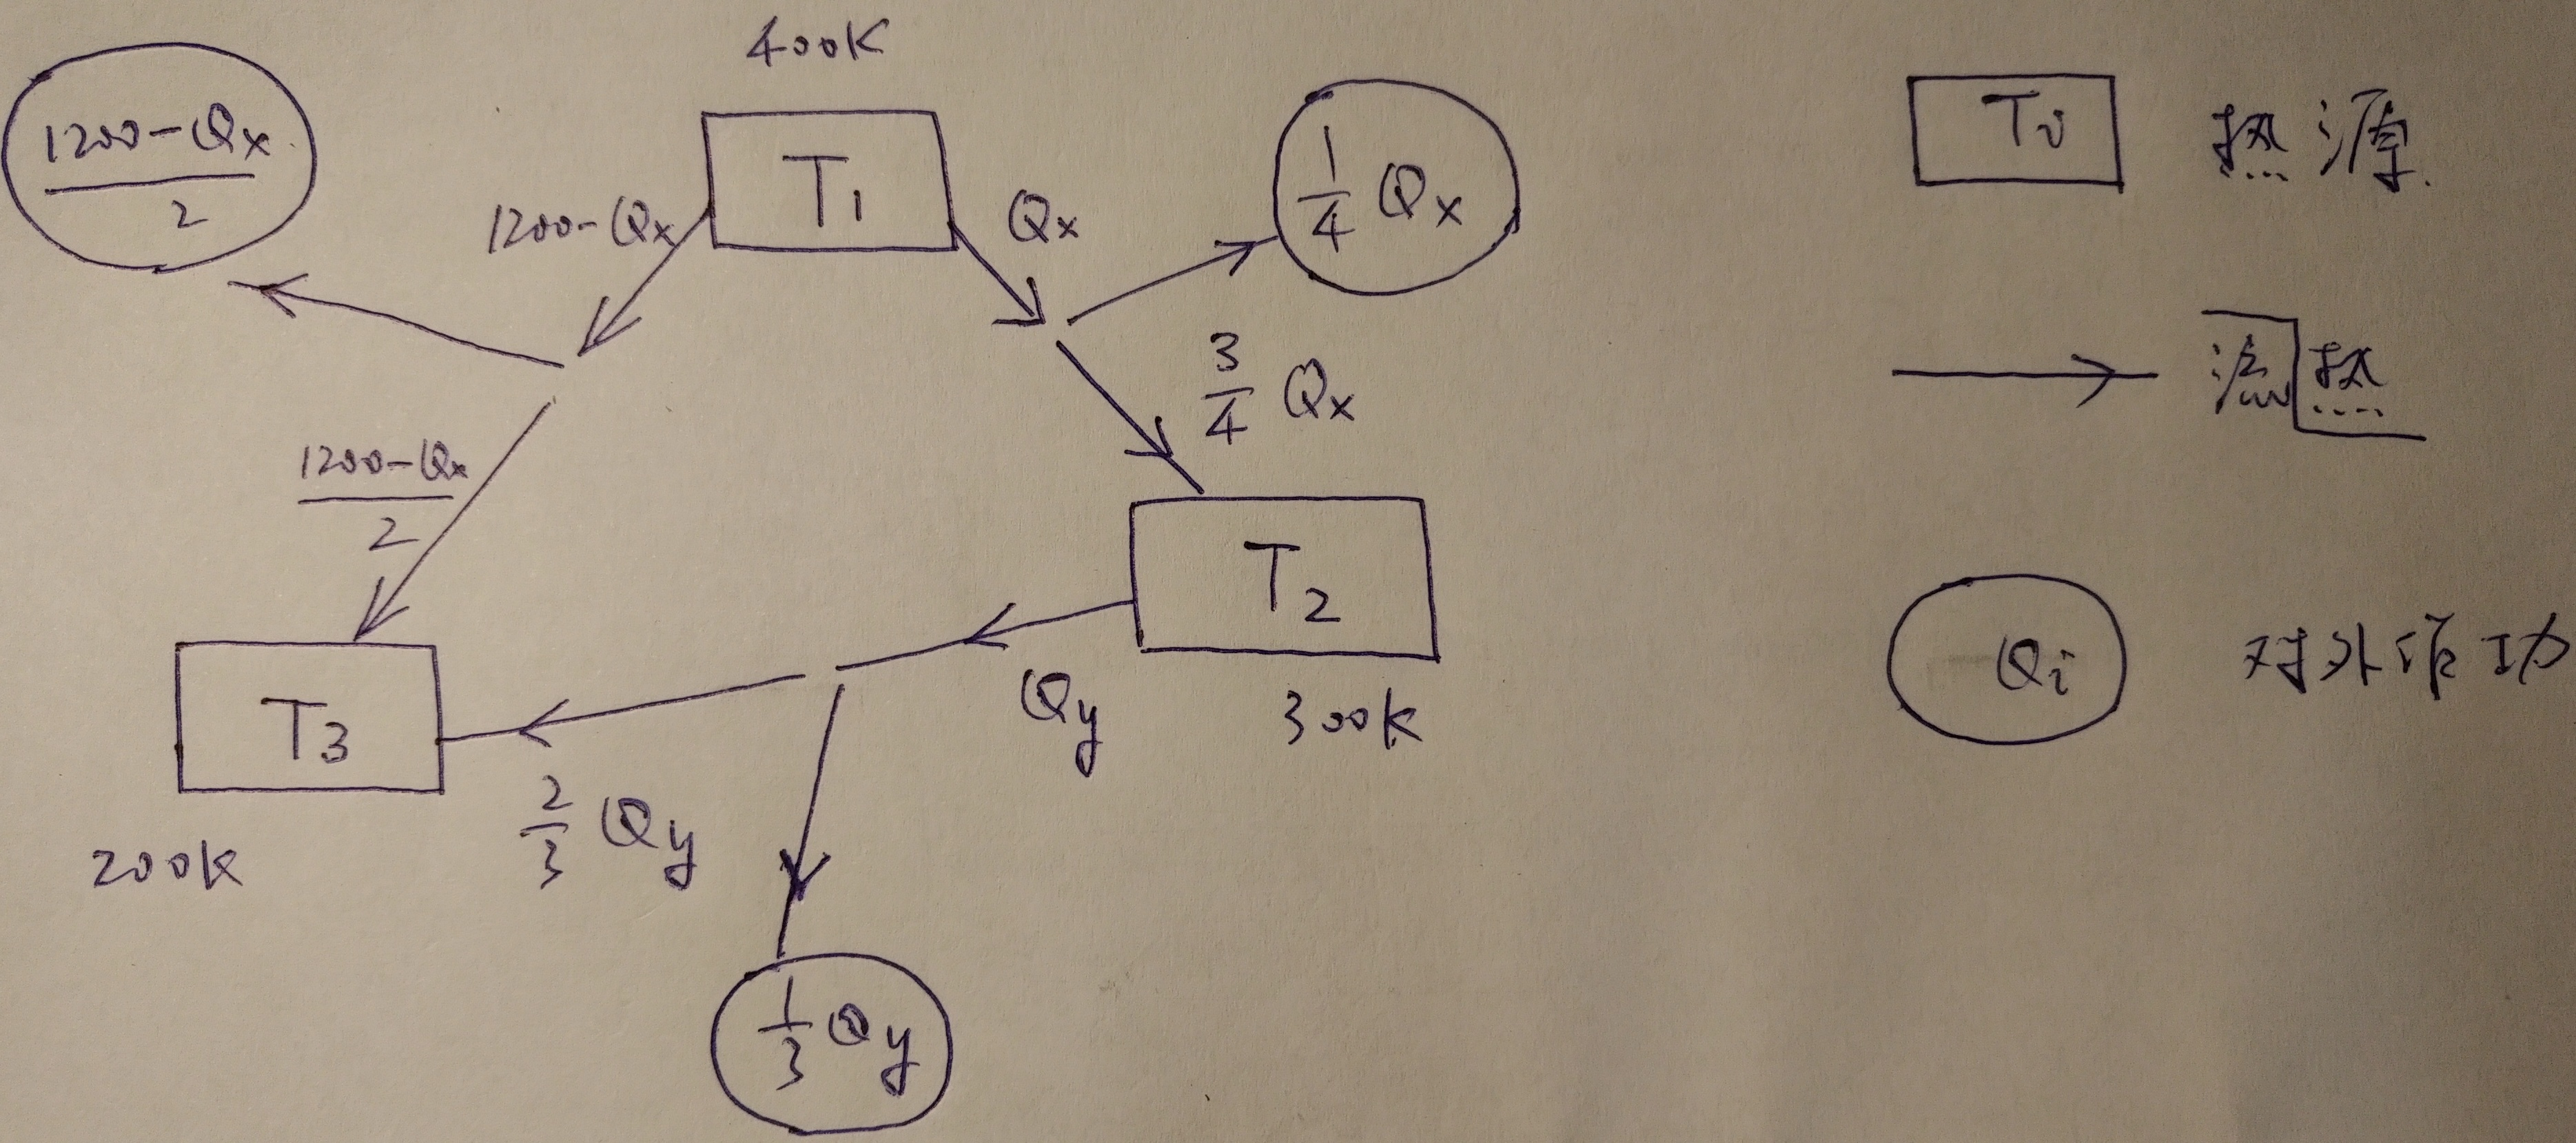
\includegraphics[width=0.5\textwidth]{heat-machine}
\end{figure}
由图, 我们有以下关系:
\begin{eqnarray*}
\frac{1200-Q_x}{2} + \frac{Q_y}{3} + \frac{Q_x}{4} = 200 & \Rightarrow & \frac{3}{4}Q_x - Q_y = 1200 \\
& \Rightarrow &
\begin{cases}
Q_2 = \frac{3}{4} Q_x - Q_y = 1200 {\rm J} \\
Q_3 = \frac{1200-Q_x}{2} + \frac{2Q_y}{3} = -200{\rm J}
\end{cases} \\
& \Rightarrow & 
\begin{cases}
\Delta S_1 = \frac{Q_1}{T_1} = \frac{-1200}{400} = -3{\rm J}/{\rm K} \\
\Delta S_2 = \frac{Q_2}{T_2} = \frac{1200}{300} = 4{\rm J}/{\rm K} \\ 
\Delta S_3 = \frac{}{Q_3}{T_3} = \frac{-200}{200} = -1{\rm J}/{\rm K} \\
\Delta S_{\text{总}} = \sum_{i = 1}^{3} \Delta S_{i} = 0{\rm J}/{\rm K} \,.
\end{cases}
\end{eqnarray*}

\subsection{习题1.23}
考虑等熵过程($ S = S_{0} $), 
\begin{eqnarray*}
W_{S_{0}} = \int_{V_{0}}^{V} p(S_{0},V') \dd V' = RS_{0} \ln \frac{V}{V_{0}} & \Rightarrow & p(S_{0}, V) = \frac{\dd W_{S_{0}}}{\dd V} = \frac{RS_{0}}{V} \\
U(S_{0},V) - U(S_{0},V_{0}) = - W_{S_{0}} & \Rightarrow & U(S_{0},V) = U_{0} - RS_{0} \ln \frac{V}{V_{0}} \,.
\end{eqnarray*}
现在考虑一个等体过程($ V, S_{0} \rightarrow V, S $) \,, 
\begin{align*}
U(S, V) - U(S_{0}, V) & = \int_{T(S_{0},V)}^{T(S,V)} T(S',V) \dd S' \\
& = \int_{S_{0}}^{S} \frac{RV_{0}}{V}\left( \frac{S'}{S_{0}} \right)^{a} \dd S' \\
& = \frac{RV_{0}S_{0}}{(a+1)V} \left[ \left( \frac{S}{S_{0}} \right)^{a+1} - 1 \right]
\end{align*}
因此,
\[ U(S, V) = \frac{RV_{0}S_{0}}{(a+1)V} \left[ \left( \frac{S}{S_{0}} \right)^{a+1} - 1 \right] - RS_{0} \ln \frac{V}{V_{0}} + U_{0} \]
又由: 
\[ \left( \frac{\partial p}{\partial S} \right)_{V} = - \left( \frac{\partial T}{\partial V} \right)_{S} = \frac{RV_{0}}{V^2} \left( \frac{S}{S_{0}} \right)^a \]
\[ \Rightarrow \quad{} p(S,V) = \frac{RV_{0}S_{0}}{(a+1)V^2} \left[ \left( \frac{S}{S_{0}} \right)^{a+1} - 1 \right] + \frac{RS_{0}}{V} \]
\[ W(S, V_{0} \rightarrow V) = \int_{V_{0}}^{V} p(S,V') \dd V' = 
\frac{RV_{0}S_{0}}{a+1} \left[ \left( \frac{S}{S_{0}} \right)^{a+1} - 1 \right] \left( \frac{1}{V_{0}} - \frac{1}{V} \right) + RS_{0} \ln \frac{V}{V_{0}} \,. \]


\newpage

\section[第二章]{第二章}

\subsection{习题2.2}
\begin{align*}
\overline{v^n} & = \frac{\int_{0}^{+\infty} v^{n+2} e^{-mv^2/2k_{B}T} \dd v}{\int_{0}^{+\infty} v^2 e^{-mv^2/2k_{B}T} \dd v} \\
& = \frac{\int_{0}^{+\infty} \left(\frac{2k_B T}{m}\right)^{\frac{n+3}{2}} s^{\frac{n+1}{2}} e^{-s} \dd s}{\int_{0}^{+\infty} \left(\frac{2k_B T}{m}\right)^{\frac{3}{2}} s^{\frac{1}{2}} e^{-s} \dd s}
\quad{} \text{变量代换: $s = \frac{mv^2}{2k_B T}$} \\
& = \left( \frac{2k_B T}{m} \right)^{\frac{n}{2}} \frac{\Gamma(\frac{n+3}{2})}{{\color{red}{\Gamma(\frac{3}{2})}}} \quad{} \text{利用$\Gamma$函数的定义} \\
& = {\color{red}{\frac{2}{\sqrt{\pi}}}} \left( \frac{2k_B T}{m} \right)^{\frac{n}{2}} \Gamma\left(\frac{n+3}{2}\right) \,.
\end{align*}

\subsection{习题2.12}
直接利用书上例$1$的结果,
\begin{align*}
F & = -Nk_{B}T \ln Z = -Nk_{B}T \big( \ln V_{1} + \frac{3}{2} \ln (2\pi m k_{B}T) \big) \,, \\
S_{\text{混前总}} & = Nk_{B} [ \ln V_1 V_2 + 3 \ln (2\pi m k_{B}T) + 3 ] + 2S_{0} \\
& = 2Nk_{B} [ \ln \sqrt{V_1 V_2} + \frac{3}{2} \ln (2\pi m k_{B}T) + \frac{3}{2} ] + 2S_{0}, \\
S_{\text{混后总}} & = 2Nk_{B} [ \ln (V_1+V_2) + \frac{3}{2} \ln (2\pi m k_{B}T) + \frac{3}{2}] + 2S_{0} \,, \\
\Delta S & = S_{\text{混后总}} - S_{\text{混前总}} \\
& = 2Nk_{B} \ln \Big( \frac{V_1 + V_2}{\sqrt{V_1 V_2}} \Big) \\
& = 2Nk_{B} \ln \Big( \frac{p_1 + p_2}{\sqrt{p_1 p_2}} \Big) \quad{} \text{利用理想气体的状态方程.}
\end{align*}

\subsection{习题2.15}
利用书上式子$2.5.16$及$2.5.22$:
\[ 
\begin{cases}
\big( \frac{\partial p}{\partial T} \big)_{v} = \big( \frac{\partial s}{\partial v} \big)_{T} = \frac{R}{v-b} \\
T \big( \frac{\partial p}{\partial T} \big)_{v} - p = \big( \frac{\partial u}{\partial v} \big)_{T} = \frac{a}{v^2}
\end{cases}
\quad{} \Rightarrow \quad{}
\big( p + \frac{a}{v^2} \big) \big( v - b \big) = RT \,.
\]

\subsection{习题2.16}
\begin{itemize}
	\item[a,b)]
	\[ \dd U = T \dd S - p \dd V = T \bigg( \frac{\partial S}{\partial p} \bigg)_{V} \dd p + \left[ T \bigg( \frac{\partial S}{\partial V} \bigg)_{p} - p \right] \dd V \]
	\[ \Rightarrow \quad{}
	\begin{cases}
	\big( \frac{\partial U}{\partial p} \big)_{V} = T \big( \frac{\partial S}{\partial p} \big)_{V} = - T \big( \frac{\partial V}{\partial T} \big)_{S} \,;\\
	\big( \frac{\partial U}{\partial V} \big)_{p} = T \big( \frac{\partial S}{\partial V} \big)_{p} - p = T \big( \frac{\partial p}{\partial T} \big)_{S} - p \,.
	\end{cases} \]
	\item[c)]
	\begin{align*}
	\dd U = T \dd S - p \dd V & = T \bigg( \frac{\partial S}{\partial T} \bigg)_{V} \dd T + \left[ T \bigg( \frac{\partial S}{\partial V} \bigg)_{T} - p \right] \dd V \\
	& \Rightarrow T \bigg( \frac{\partial S}{\partial V} \bigg)_{T} - p = \bigg( \frac{\partial U}{\partial V} \bigg)_{T} 
	= \frac{-1}{\big( \frac{\partial V}{\partial T} \big)_{U} \big( \frac{\partial T}{\partial U} \big)_{V}} \quad{} \text{and} \quad{}
	\bigg( \frac{\partial U}{\partial T} \bigg)_{V} = T \bigg( \frac{\partial S}{\partial T} \bigg)_{V} \\
	\Rightarrow \bigg( \frac{\partial T}{\partial V} \bigg)_{U} 
	& = p \bigg( \frac{\partial T}{\partial U} \bigg)_{V} - T \bigg( \frac{\partial S}{\partial V} \bigg)_{T} \bigg( \frac{\partial T}{\partial U} \bigg)_{V} \\
	& = p \bigg( \frac{\partial T}{\partial U} \bigg)_{V} - T \bigg( \frac{\partial S}{\partial V} \bigg)_{T} \frac{1}{T} \bigg( \frac{\partial T}{\partial S} \bigg)_{V} \\
	& = p \bigg( \frac{\partial T}{\partial U} \bigg)_{V} + \bigg( \frac{\partial T}{\partial V} \bigg)_{S} \\
	& = p \bigg( \frac{\partial T}{\partial U} \bigg)_{V} - T \bigg( \frac{\partial p}{\partial U} \bigg)_{V} \quad{} \text{利用$a)$结论} \,.
	\end{align*}
	\item[d)]
	\begin{align*}
	\dd H = T \dd S + V \dd p & = T \bigg( \frac{\partial S}{\partial T} \bigg)_{p} \dd T + \left[ T \bigg( \frac{\partial S}{\partial p} \bigg)_{T} + V \right] \dd p \\
	& \Rightarrow T \bigg( \frac{\partial S}{\partial p} \bigg)_{T} + V = \bigg( \frac{\partial H}{\partial p} \bigg)_{T} \quad{} \text{and} \quad{}
	\bigg( \frac{\partial H}{\partial T} \bigg)_{p} = T \bigg( \frac{\partial S}{\partial T} \bigg)_{p} \\
	\text{与c)类似的程序} & \Rightarrow \bigg( \frac{\partial T}{\partial p} \bigg)_{H} 
	= \bigg( \frac{\partial T}{\partial p} \bigg)_{S} - V \bigg( \frac{\partial T}{\partial H} \bigg)_{p}; \\
	\dd H = T \dd S + V \dd p & = T \bigg( \frac{\partial S}{\partial V} \bigg)_{p} \dd V + \left[ T \bigg( \frac{\partial S}{\partial p} \bigg)_{V} + V \right] \dd p \\
	& \Rightarrow \bigg( \frac{\partial H}{\partial V} \bigg)_{p} = T \bigg( \frac{\partial S}{\partial V} \bigg)_{p} = T \bigg( \frac{\partial p}{\partial T} \bigg)_{S}; \\
	\text{综上} & \Rightarrow \bigg( \frac{\partial T}{\partial p} \bigg)_{H} 
	= T \bigg( \frac{\partial V}{\partial H} \bigg)_{p} - V \bigg( \frac{\partial T}{\partial H} \bigg)_{p} \,.
	\end{align*}
	\item[e)]
	\begin{align*}
	\dd H = T \dd S + V \dd p & = V \bigg( \frac{\partial p}{\partial T} \bigg)_{S} \dd T + \left[ V \bigg( \frac{\partial p}{\partial S} \bigg)_{T} + T \right] \dd S \\
	& \Rightarrow V \bigg( \frac{\partial p}{\partial S} \bigg)_{T} + T = \bigg( \frac{\partial H}{\partial S} \bigg)_{T} \quad{} \text{and} \quad{}
	\bigg( \frac{\partial H}{\partial T} \bigg)_{S} = V \bigg( \frac{\partial p}{\partial T} \bigg)_{S} \\
	\Rightarrow \bigg( \frac{\partial T}{\partial S} \bigg)_{H} 
	& = - \frac{ \big( \frac{\partial H}{\partial S} \big)_{T} }{ \big( \frac{\partial H}{\partial T} \big)_{S} } \\
	& = - \frac{T}{V} \bigg( \frac{\partial T}{\partial p} \bigg)_{S} - \frac{ \big( \frac{\partial p}{\partial S} \big)_{T} }{ \big( \frac{\partial p}{\partial T} \big)_{S} } \\
	& = - \frac{T}{V} \bigg( \frac{\partial T}{\partial p} \bigg)_{S} + \frac{T}{T \big( \frac{\partial S}{\partial T} \big)_{p} } \\
	& = - \frac{T^2}{V} \bigg( \frac{\partial V}{\partial H} \bigg)_{p} + \frac{T}{C_{p}} \quad{} \text{利用了$d)$第$5$行.}
	\end{align*}
\end{itemize}

\subsection{习题2.17}
\begin{itemize}
	\item[a)]
	\begin{align*}
	\dd U = T \dd S - p \dd V & = T \bigg( \frac{\partial S}{\partial T} \bigg)_{V} \dd T + \left[ T \bigg( \frac{\partial S}{\partial V} \bigg)_{T} - p \right] \dd V \\
	& = C_{V} \dd T + \left[ T \bigg( \frac{\partial p}{\partial T} \bigg)_{V} - p \right] \dd V \,; \\
	\dd H = T \dd S + V \dd p & = T \bigg( \frac{\partial S}{\partial T} \bigg)_{p} \dd T + \left[ T \bigg( \frac{\partial S}{\partial p} \bigg)_{T} + V \right] \dd p \\
	& = C_{p} \dd T + \left[ - T \bigg( \frac{\partial V}{\partial T} \bigg)_{p} + V \right] \dd p \,.
	\end{align*}
	由全微分条件
	\begin{align*}
	\bigg( \frac{\partial C_{V}}{\partial V} \bigg)_{T} & = \left( \frac{\partial \left[ T \big( \frac{\partial p}{\partial T} \big)_{V} - p \right]}{\partial T} \right)_{V}
	= T \bigg( \frac{\partial^2 p}{\partial T^2} \bigg)_{V} \,; \\
	\bigg( \frac{\partial C_{p}}{\partial p} \bigg)_{T} & = \left( \frac{\partial \left[ - T \big( \frac{\partial V}{\partial T} \big)_{p} + V \right]}{\partial T} \right)_{p}
	= - T \bigg( \frac{\partial^2 V}{\partial T^2} \bigg)_{p} \,.
	\end{align*}
	对于理想气体而言:
	\[ \bigg( \frac{\partial C_{V}}{\partial V} \bigg)_{T} = 0 \quad{} \text{and} \quad{} \bigg( \frac{\partial C_{p}}{\partial p} \bigg)_{T} = 0, \]
	因此, 其$C_{V}, C_{p}$均仅为温度的函数. 对于范氏气体而言:
	\[ \bigg( \frac{\partial C_{V}}{\partial V} \bigg)_{T} = 0, \]
	因此, 其$C_{V}$仅为温度的函数.
	\item[b)]
	由前半小题, 我们有
	\begin{align*}
	\bigg( \frac{\partial S}{\partial V} \bigg)_{T} & = \bigg( \frac{\partial p}{\partial T} \bigg)_{V}
	= \int \frac{1}{T} \bigg( \frac{\partial C_{V}}{\partial V} \bigg)_{T} \dd T \,; \\
	\bigg( \frac{\partial S}{\partial p} \bigg)_{T} & = - \bigg( \frac{\partial V}{\partial T} \bigg)_{p}
	= \int \frac{1}{T} \bigg( \frac{\partial C_{p}}{\partial p} \bigg)_{T} \dd T \,.
	\end{align*}
	易得, 
	\begin{align*}
	S & = \int_{V} \dd V \int_{T} \frac{1}{T} \bigg( \frac{\partial C_{V}}{\partial V} \bigg)_{T} \dd T = 
	\int_{T} \frac{1}{T} \dd T {\color{cyan}{\int_{V} \dd V \bigg( \frac{\partial C_{V}}{\partial V} \bigg)_{T}}} = \int_{T} \frac{{\color{cyan}{C_{V_{0}}}}}{T} \dd T \,; \\
	S & = \int_{p} \dd p \int_{T} \frac{1}{T} \bigg( \frac{\partial C_{p}}{\partial p} \bigg)_{T} \dd T = 
	\int_{T} \frac{1}{T} \dd T {\color{red}{\int_{p} \dd p \bigg( \frac{\partial C_{p}}{\partial p} \bigg)_{T}}} = \int_{T} \frac{{\color{red}{C_{p_{0}}}}}{T} \dd T \,
	\end{align*}
	因此,
	\begin{align*}
	F & = - \int p \dd V - \int S \dd T = - \int p \dd V - \int \dd T \int \frac{C_{V_{0}}}{T} \dd T \,; \\
	G & = \int V \dd p - \int S \dd T = \int V \dd p - \int \dd T \int \frac{C_{p_{0}}}{T} \dd T \,.
	\end{align*}
\end{itemize}

\subsection{习题2.19}
能量由两部分组成, 分别是平动动能$\epsilon^{t}$与转动动能$\epsilon^{r}$. 注意到我们的目标是求状态方程, 因此我们只需要关心配分函数对$V$的依赖,
\[ Z = Z^{t} \cdot Z^{r} = \int e^{-\beta \frac{p^2}{2m}} \dd x \dd y \dd z \dd p_{x} \dd p_{y} \dd p_{z} \times 
\int e^{- \frac{\beta}{2I} \big( p_{\theta}^2 + \frac{p_{\varphi}^2}{\sin^2\!\theta} \big)} \dd \theta \dd \varphi \dd p_{\theta} \dd p_{\varphi} = V \times g(\text{不涉及$V$}).
\]
因此, 状态方程为:
\[ p = \frac{N}{\beta} \frac{\partial \ln Z}{\partial V} = \frac{N}{\beta V}, \]
即为理想气体的状态方程.

\newpage
\section{第三章}

\subsection{习题3.1}
先计算体系的配分函数
\[ P = Z^{N} = V^{N} \left[ \frac{2\pi m}{\beta} \right]^{\frac{3N}{2}},  \]
\begin{itemize}
	\item[a)]
	由此可得体系的平均能量
	\[ \bar{E} = - \frac{\partial \ln P}{\partial \beta} = \frac{3}{2} Nk_{B}T; \]
	\item[b)]
	求最概然能量$E_{p}$需写出能量的概率分布
	\[ f(E)\dd E = e^{-\Psi - \beta E} \dd \Omega(E) = e^{-\Psi - \beta E} \Omega'(E) \dd E \propto e^{-\beta E} E^{\frac{3N}{2}-1} \dd E \quad{} 
	\Rightarrow \quad{} f(E) \propto e^{-\beta E} E^{\frac{3N}{2}-1}, \]
	因此
	\[ \frac{\partial f(E)}{\partial E} \bigg|_{E=E_{p}} = 0 \quad{} \Rightarrow \quad{} E_{p} = \left(\frac{3}{2}N - 1\right) k_{B}T. \]
\end{itemize}

\subsection{习题3.3}
考虑到每个自旋有两种状态, 记为: $+1, -1$, 且分别对应了两个能量的取值: $-\mu H, +\mu H$. 体系的所有自旋的状态的选取确定了体系的一个构型(configuration), 例: 
$\{s_{i}\} = \{+1, -1, -1, -1, +1, \cdots\}$, 表示体系第$1$个自旋处于$+1$的状态, 第$2$个自旋处于$-1$的状态, 等等. 为了求体系的配分函数, 我们需要对体系的所有构型求和
\begin{align*}
P & = \sum_{\{s_{i}\}} e^{-\beta \sum_{i=1}^{N} (-1)^{(s_{i}+1)/2} \mu H} = \sum_{\{s_{i}\}} \prod_{i=1}^{N} e^{-\beta (-1)^{(s_{i}+1)/2} \mu H} \\
& = \prod_{i=1}^{N} \sum_{s_{i}=\pm1} e^{-\beta (-1)^{(s_{i}+1)/2} \mu H} = \prod_{i=1}^{N} \left( e^{-\beta \mu H} + e^{\beta \mu H} \right) \\
& = \big(2 \cosh (\beta \mu H)\big)^{N} \,,
\end{align*}
因此可得体系的内能, 熵, 热容和总磁矩分别为
\[\begin{cases}
U = -\frac{\partial}{\partial \beta} \ln P = -N \mu H \tanh(\beta \mu H)\,;\\
S = S_{0} + k_{B} \big( \ln P - \beta \frac{\partial}{\partial \beta} \ln P \big) = S_{0} + Nk_{B} \big( \ln (2\cosh \beta \mu H) - \beta \mu H \tanh \beta \mu H \big)\,;\\
C_{H} = \left( \frac{\partial U}{\partial T} \right)_{H} = - k_{B} \beta^2 \big( \frac{\partial U}{\partial \beta} \big)_{H} 
= N k_{B} \frac{(\beta \mu H)^2}{\cosh^2(\beta \mu H)}\,;\\
M = \frac{1}{\beta} \frac{\partial \ln P}{\partial H} = N \mu \tanh(\beta \mu H)\,.
\end{cases}\]

\subsection{习题3.7}
先求体系的配分函数
\[ P = V^{N} \bigg[ 4\pi \int_{0}^{+\infty} e^{-\beta c p} p^2 \dd p \bigg]^{N}  = \bigg[ \frac{8\pi V}{(c\beta)^3} \bigg]^{N}\,, \]
由此可得体系的状态方程与内能
\[\begin{cases}
p = \frac{1}{\beta} \frac{\partial \ln P}{\partial V} = \frac{N}{\beta V} \quad{} \Rightarrow \quad{} pV = Nk_{B}T\,;\\
U = -\frac{\partial \ln P}{\partial \beta} = 3Nk_{B}T.
\end{cases}\]

\subsection{习题3.11}
由能均分定理
\[ \overline{\frac{1}{2} m v_{i}^2} = \frac{1}{2} k_{B}T \quad{} \Rightarrow \quad{} \overline{v_{i}^2} = \frac{k_{B}T}{m}, \]
\begin{itemize}
	\item[a)]
	\[ \overline{v_{x}^3} \propto \int_{-\infty}^{+\infty} e^{-\beta m v_{x}^2/2} v_{x}^3 \dd v_{x} = 0\,;  \]
	\item[b)]
	\[ \overline{v_{x}^3 v_{y}} \propto \int_{-\infty}^{+\infty} e^{-\beta mv_{x}^2/2} v_{x}^3 \dd v_{x} \times \int_{-\infty}^{+\infty} e^{-\beta mv_{y}^2/2} v_{y} \dd v_{y} = 0\,; \]
	\item[c)]
	\[ \overline{v_{x}^2 v_{y}^2} = \overline{v_{x}^2} \times \overline{v_{y}^2} = \bigg( \frac{k_{B}T}{m} \bigg)^2\,; \]
	\item[d)]
	\[ \overline{(v_{x}+av_{y})^2} = \overline{v_{x}^2 + 2a v_{x} v_{y} + a^2 v_{y}^2} = \overline{v_{x}^2} + 0 + a^2 \overline{v_{y}^2} = (a^2+1) \frac{k_{B}T}{m}\,; \]
	\item[e)]
	\[ \overline{v^2 v_{x}} = \overline{v_{x}^3} + \overline{v_{y}^2 v_{x}} + \overline{v_{z}^2 v_{x}} = 0\,. \]
\end{itemize}

\subsection{习题3.12}
\begin{itemize}
	\item[a)]
	\[ \text{由能均分定理} \quad{} \Rightarrow \quad{} \bar{\epsilon} = \frac{5}{2} k_{B}T\,; \]
	\item[b)]
	\[ \overline{\frac{1}{2}m(v_{y}-v_{0})^2} = \overline{\frac{1}{2}m v_{y}^2 + \frac{1}{2} m v_{0}^2 - mv_{y}v_{0}} = \overline{\frac{1}{2}mv_{y}^2} - \frac{1}{2} m v_{0}^2 = \frac{1}{2} k_{B}T\,, \]
	因此, 我们有
	\[ \overline{\frac{1}{2}mv_{y}^2} = \frac{1}{2} k_{B}T + \frac{1}{2} m v_{0}^2\,. \]
\end{itemize}

\subsection{习题3.15}
\begin{itemize}
	\item[a)]
	\begin{align*}
	\left\langle \frac{\Omega(E)}{\Omega'(E)} \right\rangle_{\text{c.e.}} & = \int_{\Omega} e^{-\Psi - \beta E} \frac{\Omega(E)}{\Omega'(E)} \dd \Omega(E) \\
	& = \int_{0}^{+\infty} e^{-\Psi -\beta E} \Omega(E) \dd E \\
	& = - \frac{1}{\beta} \int e^{-\Psi} \Omega(E) \dd e^{-\beta E} \\
	& = - \frac{1}{\beta} e^{-\Psi - \beta E} \Omega(E) \bigg|_{E=0}^{E=+\infty} + \frac{1}{\beta} \int_{\Omega} e^{-\Psi - \beta E} \dd \Omega(E) \\
	& = \frac{1}{\beta}\,;
	\end{align*}
	\item[b)]
	由能量的概率分布
	\[ f(E) \dd E = e^{-\Psi - \beta E} \dd \Omega(E) = e^{-\Psi - \beta E} \Omega'(E) \dd E \quad{} \Rightarrow \quad{} f(E) = e^{-\Psi - \beta E} \Omega'(E), \]
	我们有
	\[ \frac{\partial f(E)}{\partial E} \bigg|_{E=E_{p}} = 0 \quad{} \Rightarrow \quad{} \frac{\Omega''(E_{p})}{\Omega'(E_{p})} = \beta\,. \]
\end{itemize}

\subsection{补充S1}
先求体系的配分函数
\[ P = Z^{N} = V^{N} \left[ \frac{2\pi m}{\beta} \right]^{\frac{3N}{2}},  \]
由此得到系统的状态方程, 内能, 熵和热容量为
\[\begin{cases}
p = \frac{1}{\beta} \frac{\partial \ln P}{\partial V} \quad{} \Rightarrow \quad{} pV = Nk_{B}T\,;\\
U = - \frac{\partial \ln P}{\partial \beta} = \frac{3}{2}Nk_{B}T\,;\\
S = S_{0} + Nk_{B} \big[ \ln V + \frac{3}{2} \ln (2\pi m k_{B} T) + \frac{3}{2} \big]\,;\\
C_{\rm v} = \frac{\partial U}{\partial T} = \frac{3}{2} Nk_B\,.
\end{cases}\]
最后, 我们来算体系的能量涨落: 
\begin{align*}
\bar{E^2} & = \int E^{2} e^{-\Psi-\beta E} {\rm d}\Omega = e^{-\Psi} \frac{\partial^{2} e^{\Psi}}{\partial \beta^{2}} = 
\frac{\partial^{2} \Psi}{\partial \beta^{2}} + \left( \frac{\partial \Psi}{\partial \beta} \right)^{2}\,\\
& \Downarrow \, \\
(E-\bar{E})^{2} & = \bar{E^{2}} - \bar{E}^{2} = \frac{\partial^{2} \Psi}{\partial \beta^{2}} = \frac{3}{2} N k_{B}^{2} T^{2}\,.
\end{align*}

\subsection{补充S2}
先求体系的配分函数
\[ Z_{g.c.} = e^{\zeta} = \sum_{N} \frac{e^{-N\alpha}}{N!} \int e^{-\beta E} \dd \Omega = 
\sum_{N} \frac{(e^{-\alpha})^N}{N!} V^N \left( \frac{2\pi m}{\beta} \right)^{\frac{3N}{2}} =
\exp\bigg[ e^{-\alpha} V \Big( \frac{2\pi m}{\beta} \Big)^{3/2} \bigg], \]
因此
\[ \zeta = e^{-\alpha} V \Big( \frac{2\pi m}{\beta} \Big)^{3/2}. \]
由此我们能得到体系的状态方程, 内能, 熵, 化学势和分子数的相对涨落
\[\begin{cases}
\bar{N} = - \frac{\partial \zeta}{\partial \alpha} = \zeta;\\
p = \frac{1}{\beta} \frac{\partial \zeta}{\partial V} = \frac{\zeta}{\beta V} \quad{} \Rightarrow \quad{} pV = \bar{N} k_{B} T;\\
U = - \frac{\partial \zeta}{\partial \beta} = \frac{3}{2} \bar{N} k_{B} T;\\
S = S_{0} + k_{B} \left( \zeta - \beta \frac{\partial \zeta}{\partial \beta} - \alpha \frac{\partial \zeta}{\partial \alpha} \right) = S_{0} + \left( \frac{5}{2} + \alpha \right) \bar{N} k_{B};\\
\mu = -\alpha k_{B} T;\\
\overline{N^2} = \sum_{N} \frac{e^{-\zeta-N\alpha}N^2}{N!} \int \cdots = e^{-\zeta} \frac{\partial^2}{\partial \alpha^2} Z_{g.c.} = 
e^{-\zeta} \frac{\partial^2}{\partial \alpha^2} e^{\zeta} = \zeta + \zeta^2;\\
\overline{(\Delta N)^2} / \bar{N}^2 = \frac{\overline{N^2}-\bar{N}^2}{\bar{N}^2} = \frac{1}{\zeta} = \frac{1}{\bar{N}}.
\end{cases}\]

\newpage
\section{第四章}

\subsection{习题4.4}
\begin{itemize}
	\item[a)]
	由书${\rm P}216$的$(4.14.3)$: $p_{F} \propto n^{1/3}$, 可知三个铜块的费米球半径相同.
	\item[b)]
	\begin{align*}
	\bar{\epsilon} & = \frac{3}{5} \mu_{0} \,; \\
	\overline{\epsilon^2} & = \frac{8 \pi V}{h^3 N} \int_{|p| \leq \sqrt{2m\mu_{0}}} \epsilon^2 p^2 \dd p 
	= \frac{8 \pi V}{h^3 N} \sqrt{2} m^{3/2} \int_{0}^{\mu_{0}} \epsilon^{5/2} \dd \epsilon 
	= \frac{8 \pi V}{h^3 N} \sqrt{2} m^{3/2} \frac{2}{7} \mu_{0}^{7/2} = \frac{3}{7} \mu_{0}^{2} \,; \\
	& \Downarrow \\
	\overline{(\epsilon-\bar{\epsilon})^2} & = \overline{\epsilon^2} - \bar{\epsilon}^2 = \frac{12}{175} \mu_{0}^2 \,.
	\end{align*}
\end{itemize}

\subsection{习题4.14}
\[ f(v) \dd v = \frac{4 \pi g V}{h^3} \frac{p^2 \dd p}{e^{(\epsilon - \mu)/k_{B}T}-1} = \frac{4 \pi g m^3 V}{h^3} \frac{v^2 \dd v}{\exp[(mv^2/2 - \mu)/k_{B}T]-1} \,; \]
\begin{align*}
\text{易得最概然速率$v_{p}$满足的方程} \qquad{} & \frac{\dd}{\dd v} \bigg( \frac{v^2}{\exp[(mv^2/2 - \mu)/k_{B}T]-1} \bigg) \bigg{|}_{v=v_{p}} = 0 \,; \\
\Rightarrow \qquad{} & v_{p}^2 = \frac{2 k_{B} T}{m} \frac{\exp[(mv_p^2/2 - \mu)/k_{B}T]-1}{\exp[(mv_p^2/2 - \mu)/k_{B}T]} \,; \\
\text{在$T>T_{c}$时, 有$\exp[(mv_p^2/2 - \mu)/k_{B}T] \gg 1$} & \\
\Rightarrow \qquad{} & v_{p} = \sqrt{\frac{2 k_{B} T}{m}} \,.
\end{align*}

\subsection{习题4.17}
考虑到膨胀前后的粒子数不变, $N_{1} = N_{2} = N$
\begin{align*}
N_{1} & = \frac{8 \pi V_{1}}{3 h^3} (2m)^{3/2} \mu_{0}^{3/2} \,; \\
N_{2} & = \frac{8 \pi V_{2}}{3 h^3} (2m)^{3/2} \mu^{3/2} \left[ 1 + \frac{\pi^2}{8}\left( \frac{k_{B} T}{\mu} \right)^2 + \cdots \right] \,,
\end{align*}
\[ \Rightarrow \quad{} \mu^{3/2} \approx \frac{V_1}{V_2} \mu_{0}^{3/2} \left[ 1 - \frac{\pi^2}{8} \left( \frac{k_{B} T}{\mu} \right)^2 \right] \,, \]
\[ \Rightarrow \quad{} \mu^{5/2} \approx \left( \frac{V_{1}}{V_{2}} \right)^{5/3} \mu_{0}^{5/2} \left[ 1 - \frac{5\pi^2}{24} \left( \frac{k_{B} T}{\mu} \right)^{2} \right] \]
显然, 膨胀前后内能也不发生改变, $E_{1} = E_{2} = E$
\begin{align*}
E_{1} & = \frac{8\pi V_{1}}{h^{3}} \sqrt{2} m^{3/2} \frac{2}{5} \mu_{0}^{5/2} \,; \\
E_{2} & = \frac{8\pi V_{2}}{h^{3}} \sqrt{2} m^{3/2} \frac{2}{5} \mu^{5/2} \left[ 1 + \frac{5\pi^{2}}{8} \left( \frac{k_{B}T}{\mu} \right)^{2} + \cdots \right] \\
& \approx \frac{8\pi V_{2}}{h^{3}} \sqrt{2} m^{3/2} \frac{2}{5} \left( \frac{V_{1}}{V_{2}} \right)^{5/3} \mu_{0}^{5/2} \left[ 1 - \frac{5\pi^2}{24} \left( \frac{k_{B} T}{\mu} \right)^{2} \right] \left[ 1 + \frac{5\pi^{2}}{8} \left( \frac{k_{B}T}{\mu} \right)^{2} + \cdots \right] \\
& \approx \frac{8\pi V_{2}}{h^{3}} \sqrt{2} m^{3/2} \frac{2}{5} \left( \frac{V_{1}}{V_{2}} \right)^{5/3} \mu_{0}^{5/2} \left[ 1 + \frac{5\pi^{2}}{12} \left( \frac{k_{B}T}{\mu} \right)^{2} \right] \,,
\end{align*}
\[ \Rightarrow \quad{} V_{1} \mu_{0}^{5/2} = V_{2} \left( \frac{V_{1}}{V_{2}} \right)^{5/3} \mu_{0}^{5/2} \left[ 1 + \frac{5\pi^{2}}{12} \left( \frac{k_{B}T}{\mu} \right)^{2} \right] \,, \]
\[ \Rightarrow \quad{} \frac{k_{B}T}{\mu} = \sqrt{ \frac{12}{5\pi^{2}} \left[ \left( \frac{V_{2}}{V_{1}} \right)^{2/3} - 1 \right] }\,. \]
最后再利用一下$\mu$粗的近似
\[ \mu \approx \left( \frac{3}{8\pi} \right)^{2/3} \frac{h^{2}}{2m} \left(\frac{N}{V_{2}} \right)^{2/3}\,, \]
\[ \Rightarrow \quad{} T = \left( \frac{3}{8\pi} \right)^{2/3} \frac{h^{2}}{2mk_{B}} \left(\frac{N}{V_{2}} \right)^{2/3} \sqrt{ \frac{12}{5\pi^{2}} \left[ \left( \frac{V_{2}}{V_{1}} \right)^{2/3} - 1 \right] }\,. \]

\subsection{习题4.19}
利用可逆绝热条件及黑体辐射的相关结论
\begin{align*}
0 & =  T \dd S = \dd U + p\dd V \,; \\
p & = \frac{1}{3} u = \frac{1}{3} a T^{4} \,; \\
U & = uV = a T^{4} V \,,
\end{align*}
将$p$与$U$代入热一公式后整理得到
\[ \dd \left( 3 \log{T} + \log{V} \right) = 0 \quad{} \Rightarrow \quad{} VT^{3} = {\rm const} \quad{} \Rightarrow \quad{} T_{\rm f} = 500 {\rm K}\,. \]

\subsection{习题4.20}
由苏书$(4.14.9)$及$(4.14.4)$
\begin{align*}
\left( \frac{\partial p}{\partial V} \right)_{T=0} & = - \frac{h^{2}}{3mV} \left( \frac{3}{8\pi} \right)^{2/3} \left( \frac{N}{V} \right)^{5/3} = - \frac{2}{3V} \epsilon_{F} n \,, \\
\Rightarrow \quad{} \kappa\rvert_{T=0} & = - \frac{1}{V} \left( \frac{\partial V}{\partial p} \right)_{T=0} = \frac{3}{2} \frac{1}{n\epsilon_{F}}\,.
\end{align*}

\subsection{习题4.25}
\begin{itemize}
	\item[a)]
	$\phi_{\vec{p}} \propto \exp{(i \vec{p} \cdot \vec{r} / \hbar)} \quad{}$ 由边界条件 $\Rightarrow \quad{} p_{\alpha} L = 2\pi\hbar n_{\alpha}\quad{} (\alpha = x, y, z)$
	\[ \Rightarrow \quad{} \epsilon = c\lvert{\vec{p}}\rvert = \frac{2\pi c\hbar}{V^{1/3}} \sqrt{n_{x}^{2}+n_{y}^{2}+n_{z}^{2}}\,. \]
	\item[b)]
	$p=\frac{U}{3V}, p_{\rm s}=\frac{U}{3NV}\,,$ $U$用玻色-爱因斯坦分布算出后再代入$\dots$
\end{itemize}

\subsection{习题4.26}
\begin{itemize}
	\item[a)]
	由各向同性, $\bar{v}_{x} = 0\,.$
	\item[b)]
	$\overline{v_{x}^{2}} = \frac{1}{3} \overline{v^{2}} = \frac{1}{3} \frac{2}{m} \bar{\epsilon} = \frac{2}{3m} \frac{3}{5} \mu_{0} = \frac{2\epsilon_{\rm F}}{5m}\,.$
\end{itemize}

\subsection{习题4.30}
\begin{align*}
\mathcal{Z} & = \sum_{n=0}^{+\infty} e^{-\beta(n+1/2)\gamma V^{-1}} = \frac{\exp{(-\beta\gamma/(2V))}}{1-\exp{(-\beta\gamma/V)}} \,; \\
\Rightarrow \quad{} \log{\mathcal{Z}} & = -\frac{1}{2} \beta\gamma V^{-1} - \log{\left(1-e^{-\beta\gamma V^{-1}}\right)} \,; \\
\Rightarrow \quad{} U & = - N \frac{\partial \log\mathcal{Z}}{\partial \beta} = \frac{N\gamma}{2V} \frac{1+e^{-\beta\gamma V^{-1}}}{1-e^{-\beta\gamma V^{-1}}} = \frac{N\gamma}{2V} \coth{(\beta\gamma/(2V))} \,; \\
\Rightarrow \quad{} C_{V} & = \left(\frac{\partial U}{\partial T}\right)_{V} = -\frac{1}{k_{B}T^{2}} \left(\frac{\partial U}{\partial \beta}\right)_{V} = \frac{N\gamma^{2}}{4k_{B}T^{2}V^{2}\sinh^{2}{(\beta\gamma/(2V))}} \,; \\
\Rightarrow \quad{} p & = \frac{N}{\beta} \frac{\partial \log\mathcal{Z}}{\partial V} = \frac{N\gamma}{2V^{2}} \coth{(\beta\gamma/(2V))} \,; \\
\Rightarrow \quad{} \bar{N}_{n} & = N \frac{e^{-\beta(n+1/2)\gamma V^{-1}}}{\sum_{n'=0}^{+\infty} e^{-\beta(n'+1/2)\gamma V^{-1}}} = N e^{-n\beta\gamma V^{-1}} \left( 1- e^{-\beta\gamma V^{-1}} \right) = 2 N e^{-(n+1/2)\beta\gamma V^{-1}} \sinh{(\beta\gamma/(2V))}\,.
\end{align*}
\begin{figure}[htbp]
\centering
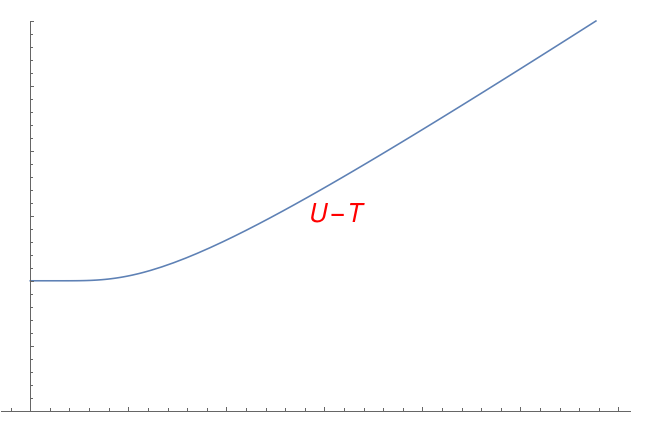
\includegraphics[width=0.35\textwidth]{ut}
\end{figure}
\begin{figure}[htbp]
\centering
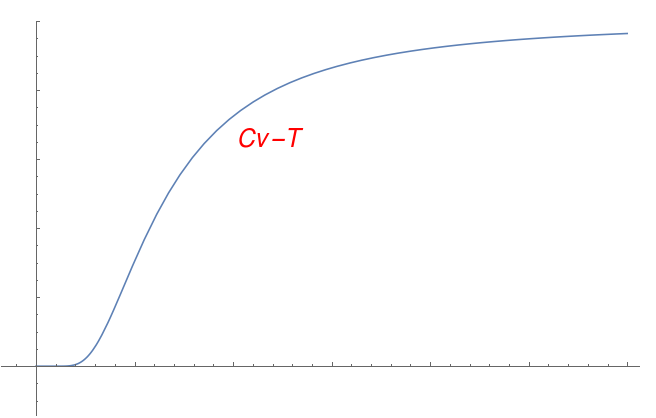
\includegraphics[width=0.35\textwidth]{cvt}
\end{figure}

\newpage
\section{第五章}

\subsection{习题5.3}
\begin{align*}
\frac{{\rm d} p}{{\rm d} T} = \frac{L}{T\Delta{v}} \quad{} \Rightarrow \quad{} \frac{{\rm d}^{2} p}{{\rm d} T^{2}} & = \frac{{\rm d} L}{{\rm d} T} \frac{1}{T\Delta{v}} - \frac{L}{\left( T \Delta{v} \right)^{2}} \frac{{\rm d}(T\Delta{v})}{{\rm d} T} \nonumber \\
& = \left[ \left( \frac{\partial{L}}{\partial{T}} \right)_{p} + \left( \frac{\partial{L}}{\partial{p}} \right)_{T} \frac{{\rm d} p}{{\rm d} T} \right] \frac{1}{T\Delta{v}} - \frac{L}{\left( T \Delta{v} \right)^{2}} \left[ \Delta{v} + T \left\{ \left( \frac{\partial{\Delta{v}}}{\partial{T}} \right)_{p} + \left( \frac{\partial{\Delta{v}}}{\partial{p}} \right)_{T} \frac{{\rm d} p}{{\rm d} T} \right\} \right]
\end{align*}
利用
\[ L=T\Delta{s} \quad{} \Rightarrow \quad{} \left( \frac{\partial{L}}{\partial{T}} \right)_{p} = \Delta{s} + \Delta{c_{p}} \quad{} \text{and} \quad{} \left( \frac{\partial{L}}{\partial{p}} \right)_{T} = T \left( \frac{\partial{\Delta{s}}}{\partial{p}} \right)_{T} {\color{red}{=}} - T \left( \frac{\partial{\Delta{v}}}{\partial{}T} \right)_{p} \quad{} {\color{red}{\text{maxwell rel.}}}\,, \]
以及近似条件
\begin{itemize}
	\item[a)] 气相体积大于液相 \qquad{} $\Delta{v} \approx v_{2}\,;$
	\item[b)] 气相定压膨胀(等温压缩)比液相大 \qquad{} $(\partial{\Delta{v}}/\partial{T})_{p} \approx (\partial{v_{2}}/\partial{T})_{p} \quad{} \text{and} \quad{} (\partial{\Delta{v}}/\partial{p})_{T} \approx (\partial{v_{2}}/\partial{p})_{T}\,;$
	\item[c)] 气相近似为理想气体.
\end{itemize}
由此得
\begin{align*}
\frac{{\rm d}^{2} p}{{\rm d} T^{2}} & = \left[ \Delta{s} + \Delta{c_{p}} - T \left( \frac{\partial{\Delta{v}}}{\partial{T}} \right)_{p} \frac{L}{T\Delta{v}} \right] \frac{1}{T\Delta{v}} - \frac{L}{(T\Delta{v})^{2}} \left[ \Delta{v} + T \left( \frac{\partial{\Delta{v}}}{\partial{T}} \right)_{p} + T \left( \frac{\partial{\Delta{v}}}{\partial{p}} \right)_{T} \frac{L}{T\Delta{v}} \right] \nonumber \\
& \approx \left[ \Delta{s} + \Delta{c_{p}} - T \left( \frac{\partial{v_{2}}}{\partial{T}} \right)_{p} \frac{L}{Tv_{2}} \right] \frac{1}{Tv_{2}} - \frac{L}{(Tv_{2})^{2}} \left[ v_{2} + T \left( \frac{\partial{v_{2}}}{\partial{T}} \right)_{p} + T \left( \frac{\partial{v_{2}}}{\partial{p}} \right)_{T} \frac{L}{Tv_{2}} \right] \nonumber \\
& \approx \left[ {\color{red}{\Delta{s}}} + \Delta{c_{p}} {\color{red}{\,-\, \frac{L}{T}}} \right] \frac{1}{Tv_{2}} - \frac{L}{(Tv_{2})^{2}} \left[ v_{2} + v_{2} - \frac{L}{p} \right] \nonumber \\
& = \frac{\Delta{c_{p}}}{Tv_{2}} - \frac{2L}{T^{2}v_{2}} + \frac{L^{2}}{T^{2}v_{2}^{2}p} \nonumber \\
& \approx \frac{\Delta{c_{p}}}{Tv_{2}} - \frac{2L}{T^{2}v_{2}} + \frac{L^{2}}{RT^{3}v_{2}}\,.
\end{align*}
最后, 代入具体的数值计算.

\subsection{习题5.8}
\begin{align*}
pv = RT \quad{} & \Rightarrow \quad{} p {\rm d}{v} + v {\rm d}{p} = R{\rm d}{T} \quad{} \Rightarrow \quad{} p \frac{{\rm d}{v}}{{\rm d}{T}} + v \frac{{\rm d}{p}}{{\rm d}T} = R \nonumber \\
& \Rightarrow \quad{} \frac{RT}{v} \frac{{\rm d}{v}}{{\rm d}{T}} + v \frac{L}{Tv} = R \quad{} \Rightarrow \quad{} {\rm d}(\ln{v}) = \frac{{\rm d}T}{T} - \frac{L{\rm d}T}{RT^{2}} \nonumber \\
& \Rightarrow \quad{} v = v_{0} T e^{L/RT}\,.
\end{align*}

\subsection{习题5.9}
\begin{align*}
\frac{{\rm d}L}{{\rm d}{T}} & = c_{p_{2}} - c_{p_{1}} + \frac{L}{T} - \left( \frac{\partial{\Delta{v}}}{\partial{T}} \right)_{p} \frac{L}{\Delta{v}} \approx c_{p_{2}} - c_{p_{1}} + \frac{L}{T} - {\color{red}{\left( \frac{\partial{v_{2}}}{\partial{T}} \right)_{p}}} \frac{L}{v_{2}} \nonumber \\
& = c_{p_{2}} - c_{p_{1}} + \frac{L}{T} - \frac{{\color{cyan}{L}}}{v_{2}} {\color{red}{\left[ \frac{v_{2}}{T} + \frac{RT}{p} \left( \frac{{\rm d}{B}}{{\rm d}{T}} p + \frac{{\rm d}{C}}{{\rm d}{T}} p^{2} + \cdots \right) \right]}} \quad{} \text{用了物态方程} \nonumber \\
& \approx c_{p_{2}} - c_{p_{1}} - {\color{cyan}{Tv_{2} \frac{{\rm d}{p}}{{\rm d}T}}} \frac{RT}{pv_{2}} \left( \frac{{\rm d}{B}}{{\rm d}{T}} p + \frac{{\rm d}{C}}{{\rm d}{T}} p^{2} + \cdots \right) \nonumber \\
& = c_{p_{2}} - c_{p_{1}} - RT^{2} \left( \frac{{\rm d}{B}}{{\rm d}{T}} \frac{{\rm d}{p}}{{\rm d}{T}} + \frac{1}{2} \frac{{\rm d}{C}}{{\rm d}{T}} \frac{{\rm d}{p^{2}}}{{\rm d}{T}} + \cdots \right) \nonumber \\
\Rightarrow \quad{} L & = L_{0} + \int_{0}^{T} (c_{p}^{0} - c_{p}^{l}) {\rm d}T - RT^{2} \left( \frac{{\rm d}{B}}{{\rm d}{T}} p + \frac{1}{2} \frac{{\rm d}{C}}{{\rm d}{T}} p^{2} + \cdots \right)\,.
\end{align*}

\subsection{习题5.10}
\begin{itemize}
	\item[a)]
	\begin{align*}
    \left(\frac{\partial{s}}{\partial{p}}\right)_{T} = -\left(\frac{\partial{v}}{\partial{T}}\right)_{p} \quad{}\Rightarrow\quad{} {\rm{d}}c_{p} & = \left(\frac{\partial{c_{p}}}{\partial{T}}\right)_{p}{\rm{d}}T + \left(\frac{\partial{c_{p}}}{\partial{p}}\right)_{T}{\rm{d}}p = \left(\frac{\partial{c_{p}}}{\partial{T}}\right)_{p}{\rm{d}}T + T\left[\frac{\partial}{\partial{p}}\left(\frac{\partial{s}}{\partial{T}}\right)_{p}\right]_{T}{\rm{d}}p \\ & = \left(\frac{\partial{c_{p}}}{\partial{T}}\right)_{p}{\rm{d}}T + T\left[\frac{\partial}{\partial{T}}\left(\frac{\partial{s}}{\partial{p}}\right)_{T}\right]_{p}{\rm{d}}p = \left(\frac{\partial{c_{p}}}{\partial{T}}\right)_{p}{\rm{d}}T - T\left[\frac{\partial}{\partial{T}}\left(\frac{\partial{v}}{\partial{T}}\right)_{p}\right]_{p}{\rm{d}}p \\ & = \left(\frac{\partial{c_{p}}}{\partial{T}}\right)_{p}{\rm{d}}T - T\left[\alpha\left(\frac{\partial{v}}{\partial{T}}\right)_{p}+v\left(\frac{\partial{\alpha}}{\partial{T}}\right)_{p}\right]{\rm{d}}p \quad{} \text{making use of $(\partial{v}/\partial{T})_{p}=\alpha{v}$}
    \end{align*}
    \begin{align*}
    {\rm{d}}c_{p1}={\rm{d}}c_{p2} \quad{}&\Rightarrow\quad{} \left(\frac{\partial{c_{p1}}}{\partial{T}}\right)_{p}{\rm{d}}T - T\left[\alpha_{1}\left(\frac{\partial{v_{1}}}{\partial{T}}\right)_{p}+v_{1}\left(\frac{\partial{\alpha_{1}}}{\partial{T}}\right)_{p}\right]{\rm{d}}p = \left(\frac{\partial{c_{p2}}}{\partial{T}}\right)_{p}{\rm{d}}T - T\left[\alpha_{2}\left(\frac{\partial{v_{2}}}{\partial{T}}\right)_{p}+v_{2}\left(\frac{\partial{\alpha_{2}}}{\partial{T}}\right)_{p}\right]{\rm{d}}p \\ &\Rightarrow\quad{} \frac{{\rm{d}}p}{{\rm{d}}T} = \frac{\Delta\left(\partial{c_{p}}/\partial{T}\right)_{p}}{Tv\Delta\left(\partial{\alpha}/\partial{T}\right)_{p}} \quad{} \text{making use of $\alpha_{1}=\alpha_{2}$, $v_{1}=v_{2}\equiv{v}$, and $(\partial{v_{1}}/\partial{T})_{p}=(\partial{v_{2}}/\partial{T})_{p}$\,.}
    \end{align*}
	\item[b)]
	\begin{align*}
	{\rm{d}\alpha} & = \left(\frac{\partial{\alpha}}{\partial{T}}\right)_{p}{\rm{d}}T + \left(\frac{\partial{\alpha}}{\partial{p}}\right)_{T}{\rm{d}}p = \left(\frac{\partial{\alpha}}{\partial{T}}\right)_{p}{\rm{d}}T + \left[\frac{\partial}{\partial{p}}\left\{\frac{1}{v}\left(\frac{\partial{v}}{\partial{T}}\right)_{p}\right\}\right]_{T}{\rm{d}}p \\ & \sim \left(\frac{\partial{\alpha}}{\partial{T}}\right)_{p}{\rm{d}}T + \frac{1}{v} \left[\frac{\partial}{\partial{p}}\left(\frac{\partial{v}}{\partial{T}}\right)_{p}\right]_{T}{\rm{d}}p \quad{} \text{inspired by the last step in a), we have omitted one term here} \\ & = \left(\frac{\partial{\alpha}}{\partial{T}}\right)_{p}{\rm{d}}T + \frac{1}{v} \left[\frac{\partial}{\partial{T}}\left(\frac{\partial{v}}{\partial{p}}\right)_{T}\right]_{p}{\rm{d}}p = \left(\frac{\partial{\alpha}}{\partial{T}}\right)_{p}{\rm{d}}T - \frac{1}{v} \left(\frac{\partial{[\kappa{v}]}}{\partial{T}}\right)_{p}{\rm{d}}p \\ & \sim \left(\frac{\partial{\alpha}}{\partial{T}}\right)_{p}{\rm{d}}T - \left(\frac{\partial{\kappa}}{\partial{T}}\right)_{p}{\rm{d}}p \quad{} \text{similarly, we have omitted one term here}
	\end{align*}
	\begin{align*}
	{\rm{d}}\alpha_{1}={\rm{d}}\alpha_{2} \quad{}&\Rightarrow\quad{} \left(\frac{\partial{\alpha_{1}}}{\partial{T}}\right)_{p}{\rm{d}}T - \left(\frac{\partial{\kappa_{1}}}{\partial{T}}\right)_{p}{\rm{d}}p = \left(\frac{\partial{\alpha_{2}}}{\partial{T}}\right)_{p}{\rm{d}}T - \left(\frac{\partial{\kappa_{2}}}{\partial{T}}\right)_{p}{\rm{d}}p \\ &\Rightarrow\quad{} \frac{{\rm{d}}p}{{\rm{d}}T}=\frac{\Delta(\partial{\alpha}/\partial{T})_{p}}{\Delta(\partial{\kappa}/\partial{T})_{p}}\,.
	\end{align*}
	\item[c)]
	\begin{align*}
	{\rm{d}}\kappa=\left(\frac{\partial{\kappa}}{\partial{T}}\right)_{p}{\rm{d}}T + \left(\frac{\partial{\kappa}}{\partial{p}}\right)_{T}{\rm{d}}p = -\left(\frac{\partial{\alpha}}{\partial{p}}\right)_{T}{\rm{d}}T + \left(\frac{\partial{\kappa}}{\partial{p}}\right)_{T}{\rm{d}}p \quad{} \text{the derivation is similar to b)}
	\end{align*}
	\begin{align*}
	{\rm{d}}\kappa_{1}={\rm{d}}\kappa_{2} \quad{}\Rightarrow\quad{} \frac{{\rm{d}}p}{{\rm{d}}T}=\frac{\Delta(\partial{\alpha}/\partial{p})_{T}}{\Delta(\partial{\kappa}/\partial{p})_{T}}\,.
	\end{align*}
	
\end{itemize}

\subsection{习题5.13}
定义跃迁矩阵[见苏书(5.6.6)]
\[ \mathcal{T} = \begin{pmatrix} e^{\beta(\epsilon+H)} & e^{-\beta\epsilon} \\ e^{-\beta\epsilon} & e^{\beta(\epsilon-H)} \end{pmatrix}\,, \]
记其本征值为$\lambda_{+} > \lambda_{-}$, 对应的本征态分别为$\lvert{+}\rangle, \lvert{-}\rangle$, 即$\mathcal{T} = \lambda_{+} \lvert{+}\rangle\langle{+}\rvert + \lambda_{-}\lvert{-}\rangle\langle{-}\rvert\,.$

由系综平均的定义式(考虑周期边界条件, $\mathcal{P}$是配分函数)
\begin{align*}
\mathcal{P}\langle{S_{i}S_{i+j}}\rangle_{{\rm Ising}} & = \sum_{S_{1}} \cdots \sum_{S_{N}} \langle{S_{1}}\rvert\mathcal{T}\lvert{S_{2}}\rangle \cdots \langle{S_{i-1}}\rvert\mathcal{T}\lvert{S_{i}}\rangle S_{i} \langle{S_{i}}\rvert\mathcal{T}\lvert{S_{i+1}}\rangle \cdots \langle{S_{i+j-1}}\rvert\mathcal{T}\lvert{S_{i+j}}\rangle S_{i+j} \langle{S_{i+j}}\rvert\mathcal{T}\lvert{S_{i+j+1}}\rangle \cdots \langle{S_{N}}\rvert\mathcal{T}\lvert{S_{1}}\rangle \nonumber \\
& = \sum_{S_{i}} \sum_{S_{i+j}} S_{i+j} \langle{S_{i+j}}\rvert\mathcal{T}^{N-j}\lvert{S_{i}}\rangle S_{i} \langle{S_{i}}\rvert\mathcal{T}^{j}\lvert{S_{i+j}}\rangle \nonumber \\
& = {\rm Tr} \left[ \sigma_{z} \mathcal{T}^{N-j} \sigma_{z} \mathcal{T}^{j} \right] \nonumber \\
& = {\rm Tr} \left[ \sigma_{z} \left( \lambda_{+}^{N-j}\lvert{+}\rangle\langle{+}\rvert + \lambda_{-}^{N-j} \lvert{-}\rangle\langle{-}\rvert \right) \sigma_{z} \left( \lambda_{+}^{j} \lvert{+}\rangle\langle{+}\rvert + \lambda_{-}^{j}\lvert{-}\rangle\langle{-}\rvert \right) \right] \nonumber \\
& = \lambda_{+}^{N} \lvert\langle{+}\rvert\sigma_{z}\lvert{+}\rangle\rvert^{2} + \lambda_{+}^{N-j}\lambda_{-}^{j} \lvert\langle{+}\rvert\sigma_{z}\lvert{-}\rangle\rvert^{2} + \lambda_{+}^{j}\lambda_{-}^{N-j} \lvert\langle{+}\rvert\sigma_{z}\lvert{-}\rangle\rvert^{2} + \lambda_{-}^{N} \lvert\langle{-}\rvert\sigma_{z}\lvert{-}\rangle\rvert^{2} \nonumber \\
\Rightarrow \quad{} \langle{S_{i}S_{i+j}}\rangle_{{\rm Ising}} & = \lvert\langle{+}\rvert\sigma_{z}\lvert{+}\rangle\rvert^{2} + \left( \frac{\lambda_{-}}{\lambda_{+}} \right)^{j} \lvert\langle{+}\rvert\sigma_{z}\lvert{-}\rangle\rvert^{2} \quad{} \text{考虑热力学极限$N\rightarrow\infty$}\,.
\end{align*}
当$H=0$时, 我们有
\begin{align*}
\lambda_{+} = 2 \cosh{(\beta\epsilon)} \qquad{} \lvert{+}\rangle = \frac{1}{\sqrt{2}} \begin{pmatrix} 1 \\ 1 \end{pmatrix} \qquad{} \text{and} \qquad{} \lambda_{-} = 2 \sinh{(\beta\epsilon)} \qquad{} \lvert{-}\rangle = \frac{1}{\sqrt{2}} \begin{pmatrix} 1 \\ -1 \end{pmatrix}\,,
\end{align*}
因此
\begin{align*}
\lim_{N\rightarrow\infty} \langle{S_{i}S_{i+j}}\rangle_{{\rm Ising}} = [\tanh{(\beta\epsilon)}]^{j}\,.
\end{align*}

\subsection{习题5.14}
\begin{align*}
\left( \frac{\partial{p}}{\partial{V}} \right)_{T} & = -\frac{RT}{(V-b)^{2}} e^{-a/RTV} + \frac{RT}{V-b} e^{-a/RTV} \frac{a}{RTV^{2}} = -\frac{p}{V-b} + \frac{ap}{RTV^{2}} \quad{} \Rightarrow \quad{} \frac{a(V-b)}{RTV^{2}}\bigg\rvert_{c} = 1 \nonumber \\
\left( \frac{\partial^{2}{p}}{\partial{V}^{2}} \right)_{T} & = -\left( \frac{\partial{p}}{\partial{V}} \right)_{T} \frac{1}{V-b} + \frac{p}{(V-b)^{2}} + \left( \frac{\partial{p}}{\partial{V}} \right)_{T} \frac{a}{RTV^{2}} - \frac{2ap}{RTV^{3}} \quad{} \Rightarrow \quad{} \frac{2a(V-b)^{2}}{RTV^{3}}\bigg\rvert_{c} = 1\,.
\end{align*}
因此
\[ \frac{pV}{RT}\bigg\rvert_{c} = \frac{2p(V-b)}{RT} \frac{RTV^{3}}{2a(V-b)^2} \frac{a(V-b)}{RTV^{2}} \bigg\rvert_{c} = 2 e^{-a/RTV} = 2 e^{-2} \approx 0.27\,. \]

\subsection{习题5.15}
\[ K_{p} = \frac{x_{\rm CO_{2}}x_{\rm H_{2}}}{x_{\rm CO}x_{\rm H_{2}O}} = \frac{0.7\times80.38}{9.46\times9.46} \approx 0.6287\,. \]

\end{document}

% 